\documentclass[11pt,a4paper]{article}

% ------------------------------------------------------------------ préambule
\usepackage[utf8]{inputenc}
\usepackage[T1]{fontenc}
\usepackage[french]{babel}
\usepackage[a4paper,margin=2.2cm]{geometry}
\usepackage{graphicx}
\usepackage{xcolor}
\usepackage{booktabs}
\usepackage{listings}
\usepackage{float}
\usepackage{caption}
\usepackage{enumitem}
\usepackage{fancyhdr}
\usepackage[hidelinks]{hyperref}

\graphicspath{{../figures/}{../figures/screenshots/}}

\definecolor{codebg}{RGB}{245,245,245}
\definecolor{codekw}{RGB}{0,90,160}
\definecolor{codecm}{RGB}{110,110,110}
\definecolor{accent}{RGB}{155,30,30}

\lstdefinestyle{sh}{
  backgroundcolor=\color{codebg}, basicstyle=\ttfamily\footnotesize,
  commentstyle=\color{codecm}\itshape, keywordstyle=\color{codekw}\bfseries,
  breaklines=true, frame=single, rulecolor=\color{gray!40},
  columns=fullflexible, keepspaces=true, showstringspaces=false,
  xleftmargin=4pt, xrightmargin=2pt, aboveskip=6pt, belowskip=6pt}
\lstset{style=sh}
\lstdefinelanguage{xmlx}{morekeywords={},morecomment=[s]{<!--}{-->},
  morestring=[b]",sensitive=false}

\captionsetup{font=small,labelfont={bf,color=accent}}

\pagestyle{fancy}\fancyhf{}
\lhead{\small TP Cybersécurité S7 - Réseau robotique ROS2}
\rhead{\small DDS non sécurisé $\rightarrow$ SROS2}
\cfoot{\small\thepage}
\renewcommand{\headrulewidth}{0.4pt}

\newcommand{\cmd}[1]{\texttt{\small #1}}

% ------------------------------------------------------------------ titre
\begin{document}
\begin{titlepage}
\centering
\IfFileExists{HESTIM.png}{%
      
\includegraphics[width=0.72\textwidth]{HESTIM.png}%
}{%
      \fbox{\parbox[c][2cm][c]{0.68\textwidth}{\centering HESTIM}}%
}\par
\vspace*{0.7cm}
{\small HESTIM - Engineering \& Business School \par}
{\small 4\textsuperscript{ème} année - Filière Cybersecurity, Semestre S7 \par}
\vspace{1.4cm}
{\Large\bfseries FASCICULE DE TRAVAUX PRATIQUES\par}
\vspace{0.6cm}
{\color{accent}\rule{0.8\textwidth}{1pt}}\par
\vspace{0.6cm}
{\LARGE\bfseries Network Lab : Sniffing and Analysing\\[2mm] a ROS2 Robot Network\par}
\vspace{0.3cm}
{\large From Unsecured DDS to SROS2 Encryption\par}
\vspace{0.4cm}
{\color{accent}\rule{0.8\textwidth}{1pt}}\par
\vspace{1.6cm}
\begin{tabular}{rl}
\textbf{Sujet} & Capture, analyse et injection de trafic DDS ; \\
 & sécurisation par SROS2 ; fingerprinting temporel\\[2mm]
\textbf{Environnement} & Docker + ROS2 Humble + Wireshark + Scapy\\[2mm]
\textbf{Réalisé par} & \begin{minipage}[t]{0.55\textwidth}\vspace{0pt}
\begin{itemize}[nosep,leftmargin=*]
  \item LUSAMOTE KIMFUTA Claudia
  \item Nom à ajouter
  \item Nom à ajouter
  \item Nom à ajouter
\end{itemize}
\end{minipage}\\
\end{tabular}

\end{titlepage}

\tableofcontents
\vspace{6mm}

% ================================================================== 1
\newpage
\section{Environnement et méthodologie}

\paragraph{Plateforme.} Le TP est réalisé sous \textbf{Windows 11} avec
\textbf{Docker Desktop}. ROS2 \textbf{Humble} s'exécute dans des conteneurs
(image \cmd{ros2-lab:humble}, basée sur \cmd{ros:humble-ros-base}) auxquels on a
ajouté \textbf{SROS2}, \textbf{Scapy}, \textbf{tcpdump}, \textbf{numpy} et
\textbf{matplotlib}. \textbf{Wireshark} est installé côté Windows pour l'analyse
des fichiers \cmd{.pcap}.

\paragraph{Topologie.} Trois conteneurs sur le réseau bridge isolé \cmd{ros2\_lab} :
\begin{itemize}[nosep]
  \item \cmd{ros2\_publisher} - \cmd{publisher\_node} : publie \cmd{/sensor\_data}
        (texte, $\approx$20\,Hz) et \cmd{/commands} (\cmd{Twist}, 2\,Hz) ;
  \item \cmd{ros2\_subscriber} - \cmd{subscriber\_node} : consomme ces topics ;
  \item \cmd{ros2\_attacker} - poste attaquant (Scapy, tcpdump, CLI \cmd{ros2}).
\end{itemize}

\paragraph{Trois corrections nécessaires à l'énoncé (spécifiques à Humble).}
Plusieurs commandes du fascicule ne fonctionnent pas telles quelles ; les
versions correctes ont été utilisées dans tout ce rapport :
\begin{enumerate}[nosep]
  \item \textbf{Capture.} Sous Windows, Wireshark ne voit pas le réseau Docker
        (il vit dans la VM de Docker Desktop). Capturer sur l'interface
        \textbf{Wi-Fi} ne montre que le trafic de l'hôte (DNS, etc.). On capture
        donc sur l'\textbf{interface bridge} \cmd{br-xxxx} de l'hôte (script
        \cmd{capture.ps1}), puis on ouvre le \cmd{.pcap} dans Wireshark.
  \item \textbf{Filtre.} \cmd{udp.port == 7400} ne montre que la découverte
        multicast. Les \emph{données} circulent en unicast sur 7410/7411. On
        utilise le filtre d'affichage \textbf{\cmd{rtps}}.
  \item \textbf{SROS2.} Le nom d'enclave doit commencer par \cmd{/}
        (\cmd{create\_enclave keystore /publisher\_node}) ; les variables
        d'environnement sont \textbf{\cmd{ROS\_SECURITY\_ENABLE}} (sans « D ») et
        \textbf{\cmd{ROS\_SECURITY\_KEYSTORE}} (et non \cmd{\_PATH}).
\end{enumerate}

% ================================================================== 2
\section{Partie A: Sniffing du trafic ROS2 non sécurisé}

\subsection{Étape 1 - Mise en place et vérification}
Le réseau et les conteneurs sont lancés, puis la communication ROS2 est vérifiée.
\begin{lstlisting}[language=bash]
docker network create --driver bridge ros2_lab
docker compose up -d
docker ps
docker exec -it ros2_attacker bash      # puis, dans le conteneur :
ros2 topic list                         # -> /sensor_data, /commands, ...
\end{lstlisting}

\begin{figure}[H]\centering
  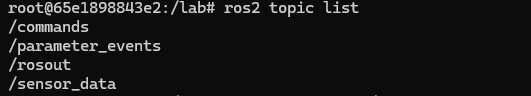
\includegraphics[width=0.78\textwidth]{a1_topic_list.png}
  \caption{\cmd{ros2 topic list} depuis le poste attaquant : sans aucune
  authentification, les topics \cmd{/sensor\_data} et \cmd{/commands} sont
  immédiatement visibles.}
\end{figure}

\begin{figure}[H]\centering
  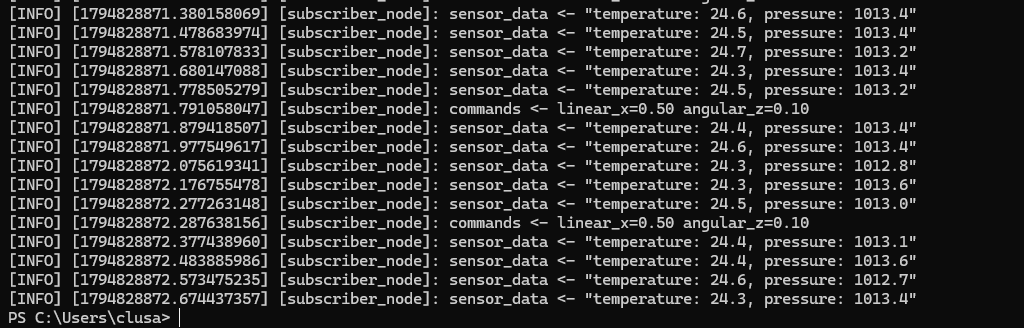
\includegraphics[width=0.92\textwidth]{a1_subscriber_log.png}
  \caption{Le \cmd{subscriber\_node} reçoit les mesures en clair
  (\cmd{temperature}, \cmd{pressure}) et les consignes (\cmd{linear\_x},
  \cmd{angular\_z}).}
\end{figure}

\subsection{Étape 2 - Capture Wireshark}
Capture de 60\,s sur l'interface bridge :
\begin{lstlisting}[language=bash]
.\capture.ps1 -Name unsecured -Seconds 60    # -> captures\unsecured.pcap
\end{lstlisting}

\noindent\textbf{Mesures demandées} (fichier \cmd{unsecured.pcap}, via
\cmd{capinfos}) :
\begin{center}\small
\begin{tabular}{@{}lll@{}}
\toprule
Paquets & Débit & Taille moyenne \\
\midrule
907 paquets en 58,9\,s & \textbf{$\approx$15,4 paquets/s} & \textbf{171,6 octets} \\
\bottomrule
\end{tabular}
\end{center}
Répartition par port : 827 paquets vers 7411 (données unicast), 40 vers 7410 et
40 vers 7400 (découverte SPDP multicast) — ce qui confirme que le filtre
\cmd{udp.port == 7400} de l'énoncé passerait à côté de l'essentiel du trafic.

\subsection{Étape 3 - Extraction des noms de topics (découverte SPDP/SEDP)}
Les annonces de découverte transportent, \textbf{en clair}, les noms de topics,
les types de messages et l'identité des nœuds. Dans Wireshark : filtre
\cmd{rtps.param.topicName}.

\begin{figure}[H]\centering
  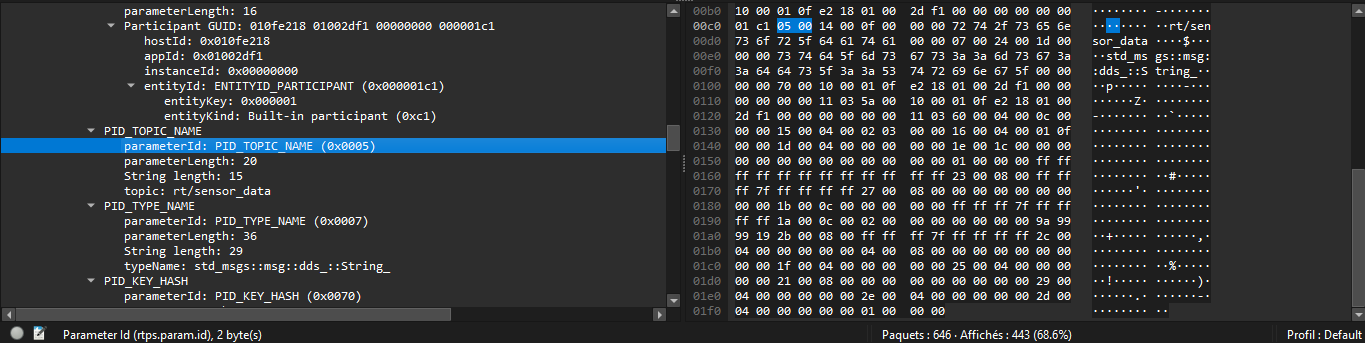
\includegraphics[width=0.99\textwidth]{a3_topic_type.png}
  \caption{Paquet de découverte \cmd{DATA(w)} déplié : \cmd{PID\_TOPIC\_NAME =
  rt/sensor\_data} et \cmd{PID\_TYPE\_NAME = std\_msgs::msg::dds\_::String\_},
  lisibles en clair (y compris dans la vue hexadécimale à droite).}
\end{figure}

\begin{center}\small
\begin{tabular}{@{}lll@{}}
\toprule
Topic (DDS) & Type de message & Rôle \\
\midrule
\cmd{rt/sensor\_data} & \cmd{std\_msgs/msg/String} & mesures capteur \\
\cmd{rt/commands} & \cmd{geometry\_msgs/msg/Twist} & consignes de vitesse \\
\cmd{rt/rosout} & \cmd{rcl\_interfaces/msg/Log} & journaux (interne ROS2) \\
\cmd{rt/parameter\_events} & \cmd{rcl\_interfaces/msg/ParameterEvent} & interne ROS2 \\
\cmd{rq/.../...Request} & services de paramètres & révèlent le nom des nœuds \\
\bottomrule
\end{tabular}
\end{center}

\noindent\textbf{Réponse attendue :} un attaquant cartographie tout le système
(qui publie, qui écoute, sur quels topics, avec quels types) \emph{uniquement} à
partir du trafic de découverte, \textbf{sans intercepter une seule donnée}.

\subsection{Étape 4 - Lecture du contenu des messages}
Les paquets de données (filtre \cmd{rtps.sm.id == 0x15}) exposent la charge utile
en clair.

\begin{figure}[H]\centering
  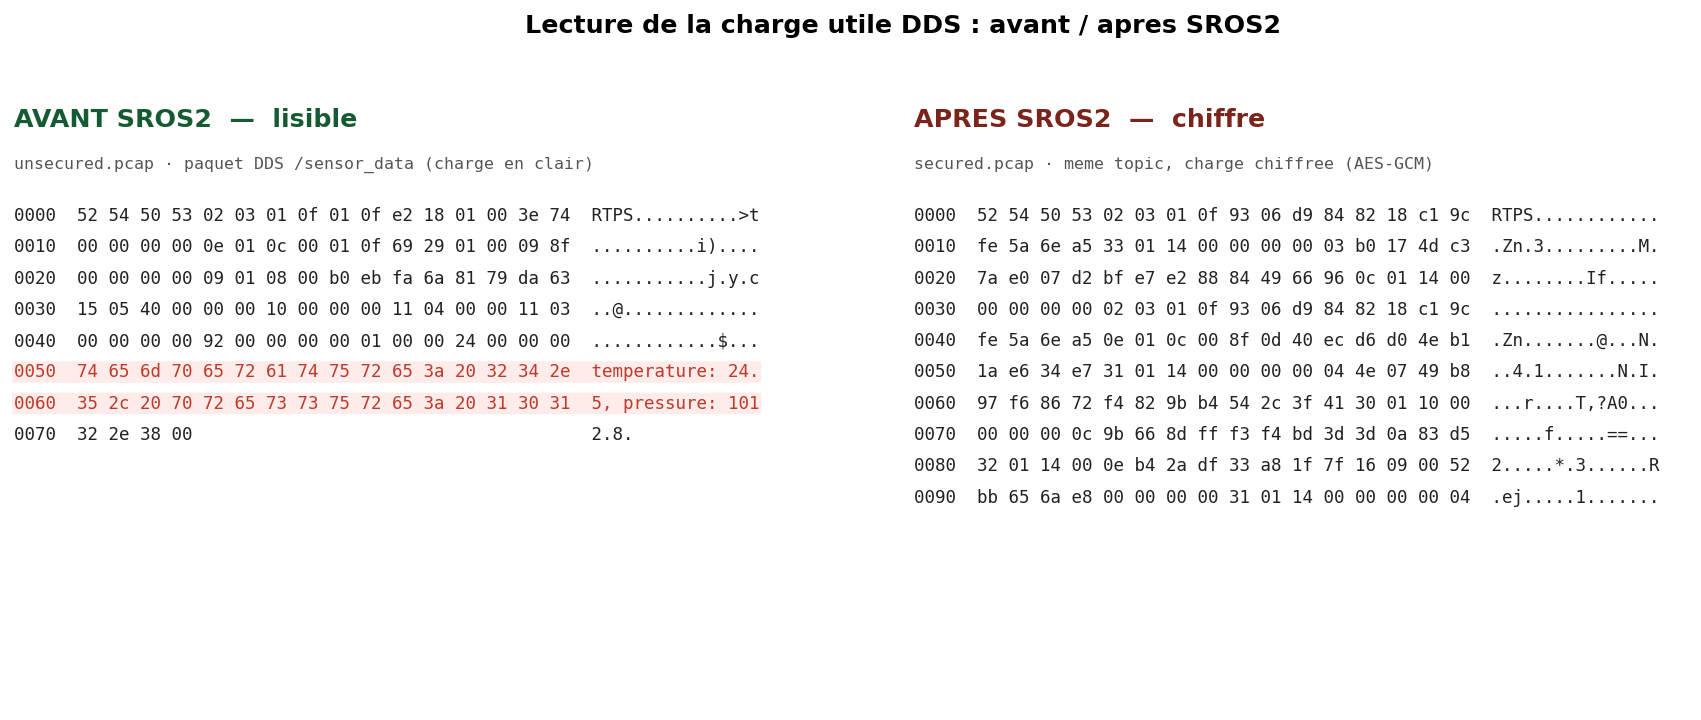
\includegraphics[width=\textwidth]{fig_payload_comparaison.png}
  \caption{À gauche : octets d'un paquet \cmd{/sensor\_data} de
  \cmd{unsecured.pcap}. La chaîne \cmd{"temperature: 24.5, pressure: 1012.8"}
  est directement lisible (surlignée). À droite : le même topic sous SROS2
  (Partie B), charge chiffrée et illisible.}
\end{figure}

\noindent\textbf{Données sensibles lisibles :} mesures de capteurs (température,
pression) et consignes de déplacement du robot (\cmd{linear\_x},
\cmd{angular\_z}).\\
\textbf{Conséquence physique :} l'attaquant connaît en temps réel l'état de
l'environnement et les mouvements du robot ; il peut le suivre, anticiper ses
trajectoires, et surtout préparer une injection crédible (il connaît les plages
de valeurs normales).

\subsection{Étape 5 - Injection de paquets (spoofing) avec Scapy}
\textbf{Principe de l'attaque} (script \cmd{inject\_dds.py}) : DDS sans SROS2
n'offre ni authentification ni chiffrement. L'attaquant (1) capture un paquet
\cmd{DATA} légitime, (2) en recopie l'en-tête — \emph{même GUID d'écrivain}, le
subscriber le croit donc légitime, (3) remplace la valeur du capteur
(\cmd{24.5}~$\rightarrow$~\cmd{99.9}), (4) \textbf{incrémente le numéro de
séquence (SN)} pour que le lecteur BEST\_EFFORT accepte l'échantillon comme
« nouveau », (5) ré-émet la trame.

\begin{lstlisting}[language=bash]
python3 inject_dds.py --iface br-xxxx --count 8
# [*] Valeur reelle : temperature: 24.5, pressure: 1013.4
# SN 191 -> 691 (le subscriber BEST_EFFORT accepte un SN superieur)
\end{lstlisting}

\begin{figure}[H]\centering
  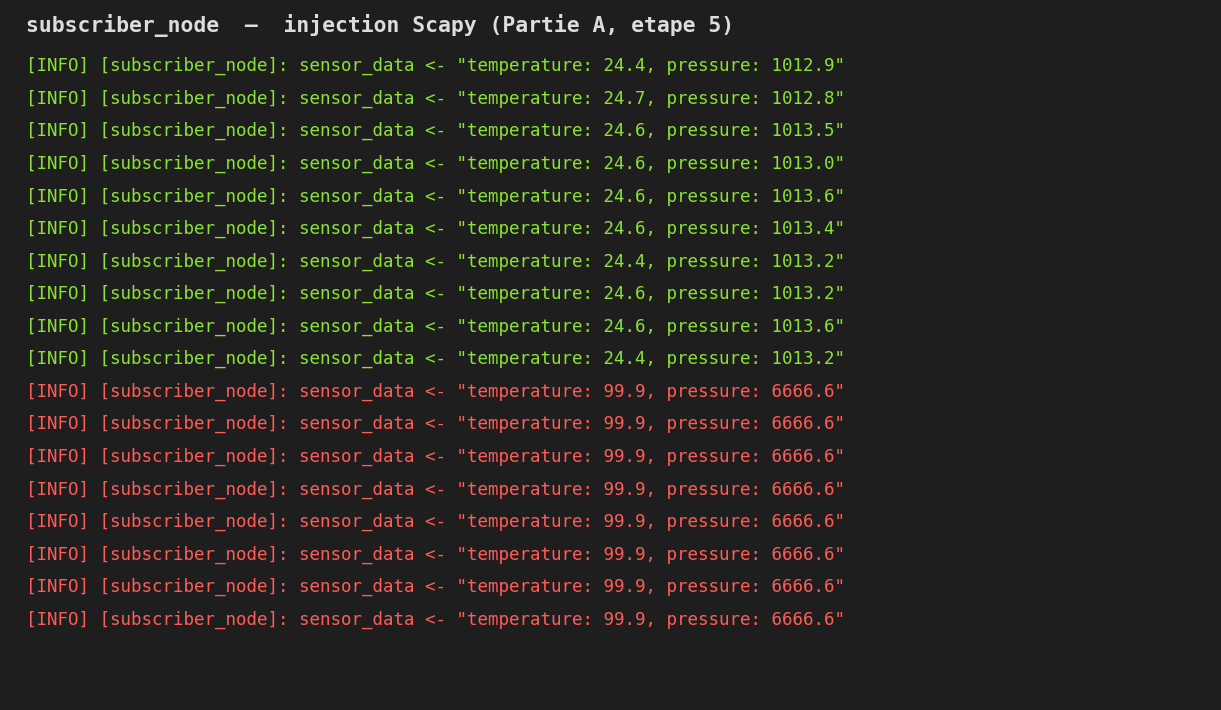
\includegraphics[width=0.97\textwidth]{fig_subscriber_spoofe.png}
  \caption{Preuve du spoofing : après l'injection, le \cmd{subscriber\_node}
  affiche la \textbf{fausse} valeur \cmd{temperature: 99.9, pressure: 6666.6}.
  Le flux réel est même évincé (l'attaquant a pris la main sur le topic).}
\end{figure}

\noindent\textbf{Si c'était un vrai robot :} une fausse mesure de capteur conduit
à une décision erronée du système de contrôle (p.\,ex. croire la température
critique, stopper un process, ou au contraire ignorer un danger réel)
$\rightarrow$ \textbf{danger physique}. On a aussi observé un effet de déni de
service : le flux légitime est écrasé par le flux usurpé.

\subsection{Étape 6 - Synthèse Partie A}
\begin{center}\small
\begin{tabular}{@{}p{3.2cm}p{11cm}@{}}
\toprule
Ce qu'un attaquant \textbf{voit} & topologie complète (nœuds, topics, types),
mesures et consignes en clair, fréquences d'émission. \\
Ce qu'un attaquant \textbf{fait} & usurpe des mesures (spoofing), évince le flux
légitime (DoS), pourrait rejouer/altérer des commandes. \\
\bottomrule
\end{tabular}
\end{center}

% ================================================================== 3
\section{Partie B: SROS2 et fingerprinting}

\subsection{Étape 1 - Création du keystore et des enclaves}
\begin{lstlisting}[language=bash]
ros2 security create_keystore keystore
ros2 security create_enclave keystore /publisher_node     # NB : le slash initial
ros2 security create_enclave keystore /subscriber_node
# variables (Humble) : ROS_SECURITY_ENABLE=true et ROS_SECURITY_KEYSTORE=<...>/keystore
\end{lstlisting}
Chaque enclave contient un certificat X.509 (\cmd{cert.pem}), une clé privée
(\cmd{key.pem}), les CA d'identité et de permissions, la gouvernance signée et
le fichier de permissions signé.

\subsection{Étape 2 - Gouvernance et permissions}
\textbf{Gouvernance} (\cmd{sros2/governance.xml}) — tout le domaine est
authentifié et chiffré :
\begin{lstlisting}[language=bash]
<allow_unauthenticated_participants>false</allow_unauthenticated_participants>
<enable_join_access_control>true</enable_join_access_control>
<discovery_protection_kind>ENCRYPT</discovery_protection_kind>
<rtps_protection_kind>SIGN</rtps_protection_kind>
<metadata_protection_kind>ENCRYPT</metadata_protection_kind>
<data_protection_kind>ENCRYPT</data_protection_kind>
\end{lstlisting}

\noindent\textbf{Matrice d'accès} (\cmd{sros2/tp\_policy.xml}), appliquée via
\cmd{ros2 security create\_permission} / \cmd{generate\_artifacts} :
\begin{center}\small
\begin{tabular}{@{}lccc@{}}
\toprule
Identité & \cmd{/sensor\_data} & \cmd{/commands} & Autres topics \\
\midrule
\cmd{publisher\_node}  & \textbf{publier}   & \textcolor{accent}{refusé} & refusé \\
\cmd{subscriber\_node} & \textbf{s'abonner} & \textcolor{accent}{refusé} & refusé \\
toute autre identité   & \multicolumn{3}{c}{\textcolor{accent}{refusé (pas de certificat valide)}} \\
\bottomrule
\end{tabular}
\end{center}
Vérification que la restriction est réelle : le fichier de permissions généré
pour \cmd{publisher\_node} autorise \cmd{rt/sensor\_data} mais \textbf{ne contient
pas} \cmd{rt/commands}. Lorsqu'un nœud tente une opération hors de ses droits, la
couche de sécurité DDS refuse la création du reader/writer
(\emph{« Problem creating associated Reader »}).

\subsection{Étape 3 - Re-capture chiffrée}
\begin{lstlisting}[language=bash]
$env:ROS_SECURITY_ENABLE = "true"
docker compose up -d --force-recreate publisher subscriber
.\capture.ps1 -Name secured -Seconds 60     # -> captures\secured.pcap
\end{lstlisting}
Le \cmd{subscriber\_node} reçoit toujours les données (il est authentifié), mais
l'analyse de \cmd{secured.pcap} donne \textbf{0 occurrence} de la chaîne
\cmd{temperature} : la charge est chiffrée (voir le volet droit de la figure~3).
On distingue encore la structure RTPS, mais plus le contenu.

\subsection{Étape 4 - Le spoofing et l'écoute sont bloqués}
\begin{figure}[H]\centering
  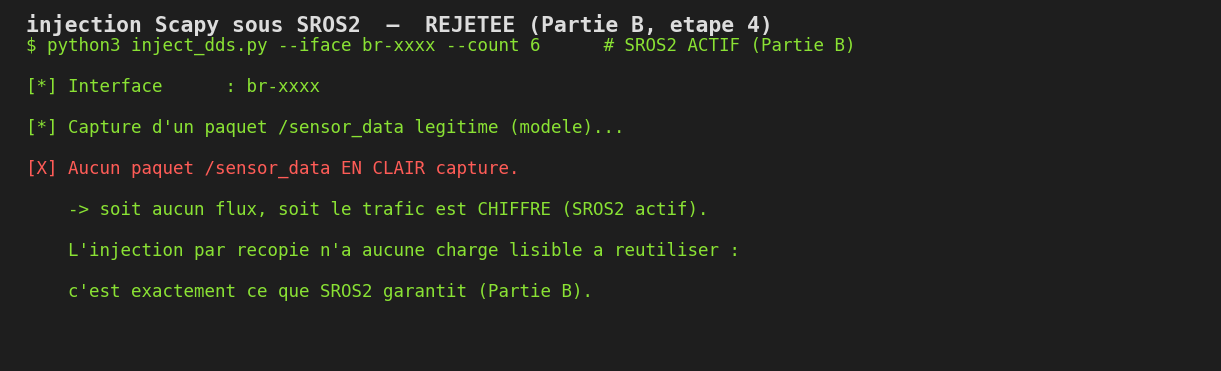
\includegraphics[width=0.84\textwidth]{fig_injection_bloquee.png}\\[2mm]
  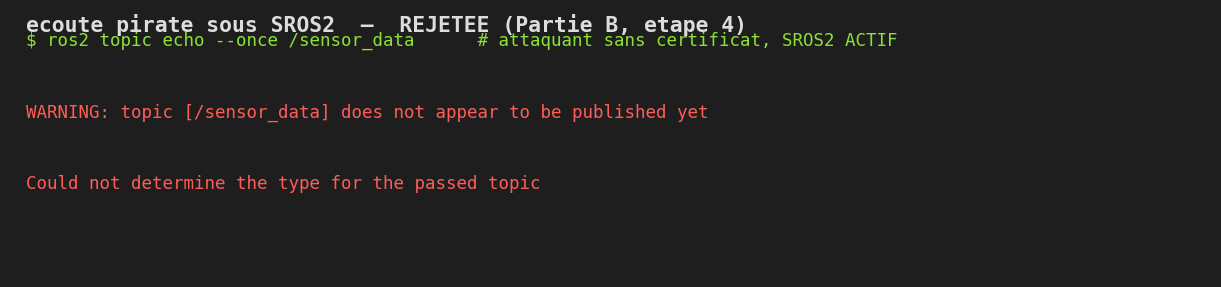
\includegraphics[width=0.84\textwidth]{fig_ecoute_bloquee.png}
  \caption{Sous SROS2 : (haut) l'injection Scapy n'a aucune charge en clair à
  recopier et la trame forgée, sans signature valide, est rejetée ; (bas) un
  attaquant sans certificat ne peut même pas déterminer le type du topic.}
\end{figure}
\noindent\textbf{Analyse :} l'authentification (certificats X.509) + le contrôle
d'accès (permissions) stoppent l'usurpation. La catégorie \textbf{STRIDE « S »
(Spoofing) est mitigée} ; le chiffrement traite « I » (Information disclosure) et
la signature RTPS traite « T » (Tampering).

\subsection{Étape 5 - Fingerprinting temporel (canal auxiliaire)}
Même chiffré, l'\emph{espacement} des paquets reste visible. Le script
\cmd{timing\_analysis.py} mesure les intervalles inter-paquets pour deux états :

\begin{figure}[H]\centering
  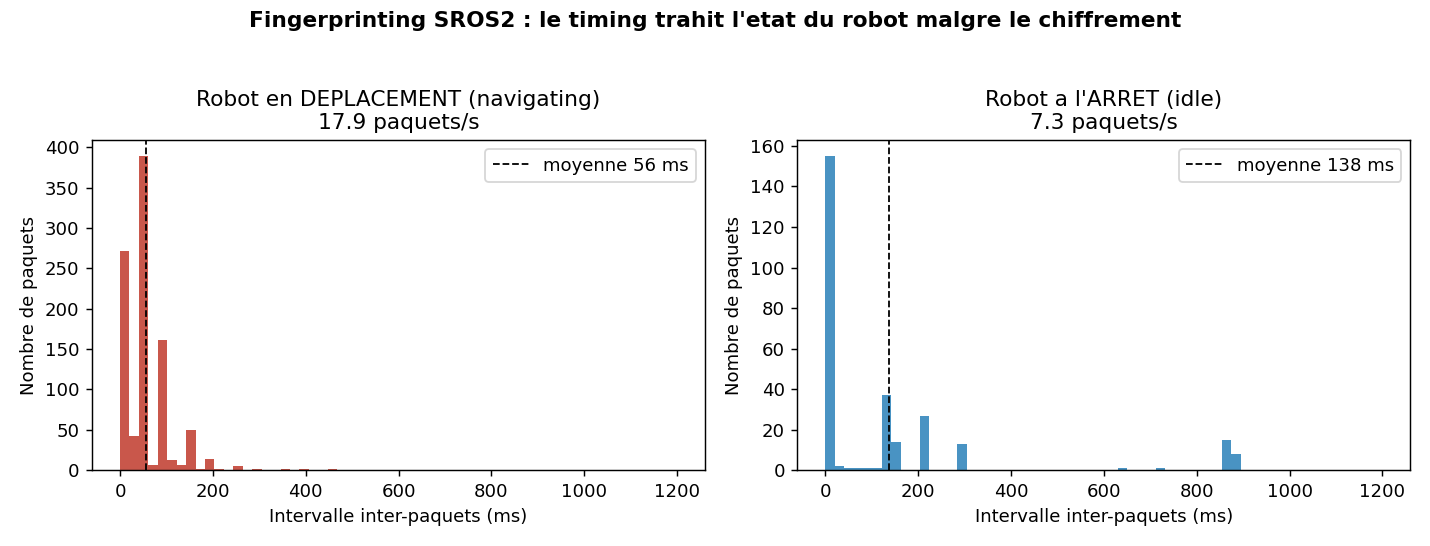
\includegraphics[width=\textwidth]{timing_plot.png}
  \caption{Distribution des intervalles inter-paquets (trafic \textbf{chiffré}).
  Les deux états sont nettement séparables sans jamais déchiffrer.}
\end{figure}

\begin{center}\small
\begin{tabular}{@{}lccc@{}}
\toprule
État & Débit & Intervalle moyen & Écart-type \\
\midrule
Robot en déplacement (navigating) & 17,9 pq/s & 55,8\,ms & 52,2\,ms \\
Robot à l'arrêt (idle) & 7,3 pq/s & 138,0\,ms & 244,2\,ms \\
\bottomrule
\end{tabular}
\end{center}

\noindent\textbf{Réponse :} oui, le débit et la forme de la distribution
trahissent l'activité du robot (déplacement vs arrêt) malgré le chiffrement.
C'est une \textbf{attaque par canal auxiliaire}. \textbf{Défenses :} rembourrage
des paquets à taille constante (\emph{packet padding}), émission à cadence fixe
avec trafic factice (\emph{constant-rate / dummy traffic}), et obfuscation
temporelle (jitter aléatoire), au prix d'un surcoût en bande passante et en
latence.

% ================================================================== 4
\section{Recommandations: au-delà de SROS2}
SROS2 protège l'authentification, l'intégrité et la confidentialité au niveau
DDS, mais ne couvre pas tout :
\begin{itemize}[nosep]
  \item \textbf{Segmentation réseau} : VLAN dédié robot, pare-feu, et
        chiffrement de niveau liaison/réseau (MACsec, IPsec) pour masquer aussi
        les métadonnées de timing.
  \item \textbf{Anti-fingerprinting} : padding et cadence constante sur les
        topics sensibles.
  \item \textbf{Gestion des clés} : rotation des certificats, CA protégée (HSM),
        révocation ; ne jamais embarquer les clés privées en clair.
  \item \textbf{Moindre privilège} : permissions par nœud au plus juste (ce TP),
        revues régulièrement.
  \item \textbf{Supervision} : IDS réseau, détection d'anomalies de débit/SN,
        journalisation des refus de sécurité DDS.
  \item \textbf{Durcissement système} : images à jour, \emph{secure boot},
        intégrité du firmware des capteurs, sécurité physique des accès réseau.
  \item \textbf{Disponibilité} : limitation de débit et redondance contre le DoS
        (observé en Partie A).
\end{itemize}

% ================================================================== 5
\section{Conclusion}
La Partie A montre qu'un réseau robotique ROS2 \emph{sans} SROS2 est totalement
exposé : cartographie par la découverte, lecture des mesures et des commandes en
clair, et usurpation de capteur réussie (fausse valeur acceptée par le
subscriber, avec éviction du flux légitime). La Partie B montre que SROS2
(authentification X.509, chiffrement AES-GCM, contrôle d'accès par permissions)
rétablit confidentialité, intégrité et authenticité : le contenu devient
illisible et le spoofing est rejeté. Il subsiste toutefois un \textbf{canal
auxiliaire temporel} : le \emph{timing} des paquets chiffrés révèle encore
l'état du robot, ce qui justifie des contre-mesures complémentaires (padding,
cadence constante, chiffrement de niveau réseau).

\appendix
\section{Livrables joints}
\begin{itemize}[nosep]
  \item \cmd{ros2\_lab/captures/} : \cmd{unsecured.pcap}, \cmd{discovery.pcap},
        \cmd{secured.pcap}, \cmd{navigating.pcap}, \cmd{idle.pcap}.
  \item \cmd{ros2\_lab/sros2/} : \cmd{governance.xml}, \cmd{tp\_policy.xml},
        \cmd{permissions\_publisher.xml}, \cmd{permissions\_subscriber.xml} ;
        keystore complet dans \cmd{ros2\_lab/keystore/}.
  \item \cmd{scripts/} : \cmd{inject\_dds.py}, \cmd{timing\_analysis.py},
        \cmd{gen\_figures.py}.
  \item \cmd{figures/} : graphe de fingerprinting, comparaison clair/chiffré,
        preuves d'injection, captures d'écran annotées.
\end{itemize}

\end{document}
